\documentclass[14pt]{beamer}

\usepackage{url}
\usepackage{graphicx}

\usefonttheme{structurebold}
\setbeamercolor{background canvas}{bg=black}
\setbeamercolor{normal text}{fg=white}
\setbeamercolor{structure}{fg=white}
\setbeamertemplate{navigation symbols}{}

\title{Uncommon things you do}
\author{
        Chris Lamb \\
        \vskip 6mm
        \tiny{\url{https://chris-lamb.co.uk}}
}
\date{}

\begin{document}

\centering

\frame{
	\titlepage
    
\includegraphics[width=15mm]{img/thread.png}
}

\frame {}

\frame {
    Pulse \\
    \vskip 1em
    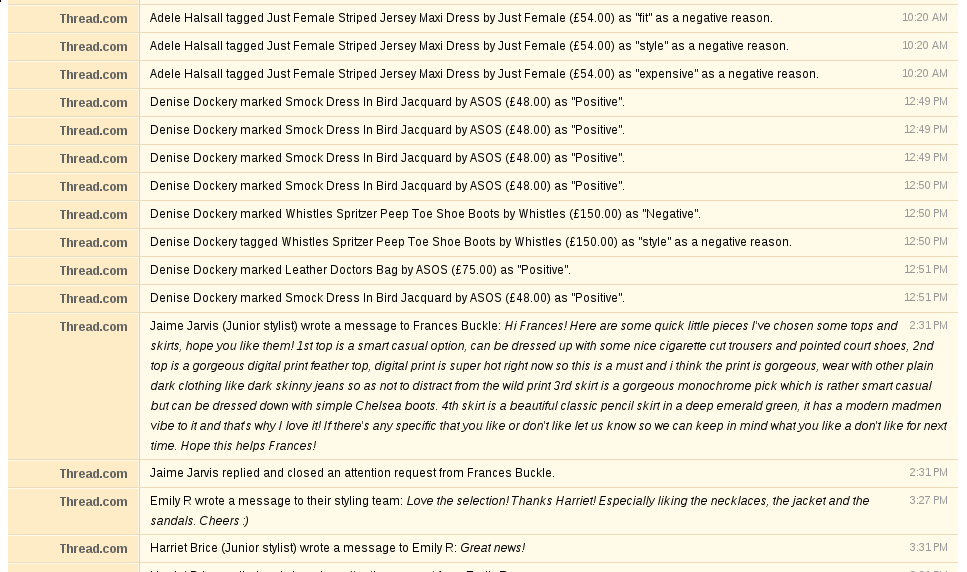
\includegraphics[width=100mm]{img/pulse.png}
}

\frame {
    Pulse history \\
    \vskip 1em
    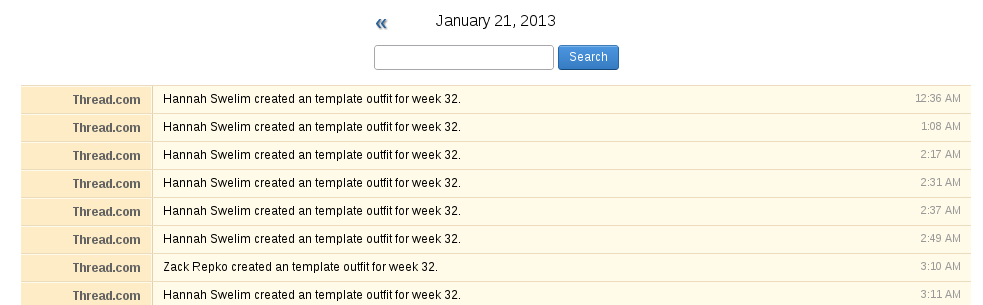
\includegraphics[width=100mm]{img/pulse-history.png}
}

\frame {
    Debian packaging
}

\frame {
    Auto-login links in emails \\
    \vskip 1em
    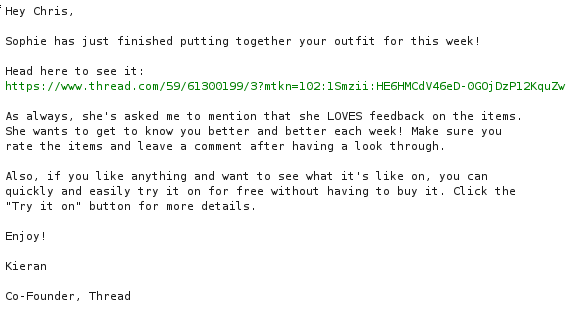
\includegraphics[width=100mm]{img/auto-login.png}
}

\frame {
    \begin{itemize}
        \item \url{https://github.com/playfire/django-autologin}
        \item Allow login link to any URL
        \item Salted HMAC implementation - no state
        \item Token includes timestamp so tokens expire
        \item Customisable salt fields - default: user.password (hashed)
        \item Tokens can be re-used (feature?)
    \end{itemize}
}

\frame{
    Cutting edge version of framework
}

\frame {}

\end{document}
